\subsection{Superficial elements}

In this section, let q denote an ideal of A contained in the radical of A, and let M be a nonzero finitely generated A-module such that M/qM has finite length.

PROPOSITION 8. --- Let \(\delta > 0\) be an integer, \(x\) an element of \(\mathfrak{q}^{\delta}\) , \(\xi\) its class in \(\mathrm{gr}_{\delta}(\mathbf{A}) = \mathfrak{q}^{\delta}/\mathfrak{q}^{\delta+1}\) , and \(\varphi\) denote multiplication by \(\xi\) in the \(\mathrm{gr}(\mathbf{A})\) -module \(\mathrm{gr}(\mathbf{M})\) .

\begin{enumerate}
\def\labelenumi{\alph{enumi})}
\item
  The dimension of the A-module M/xM is equal to \(\dim_{\mathbf{A}}(\mathbf{M})\) or to \(\dim_{\mathbf{A}}(\mathbf{M}) - 1\) . In the second case, we have \(e_{\mathfrak{q}}(\mathbf{M}/x\mathbf{M}) \geqslant \delta e_{\mathfrak{q}}(\mathbf{M})\) .
\item
  Suppose that we have \(\dim_{\mathbf{A}}(\mathbf{M}) \geqslant 1\) and that the kernel of \(\varphi\) is of finite length over A/q. Then we have \(\dim_{\mathbf{A}}(\mathbf{M}/x\mathbf{M}) = \dim_{\mathbf{A}}(\mathbf{M}) - 1\) . Moreover:
\end{enumerate}

\begin{enumerate}
\def\labelenumi{(\roman{enumi})}
\item
  If \(\dim_{\mathbf{A}}(\mathbf{M}) > 1\) , one has \(e_{\mathfrak{q}}(\mathbf{M} / x\mathbf{M}) = \delta e_{\mathfrak{q}}(\mathbf{M})\) .
\item
  If \(\dim_{\mathbf{A}}(\mathbf{M}) = 1\) , one has, for every integer \(n \geqslant 0\)
\end{enumerate}

\[
n \delta e _ {\mathfrak {q}} (\mathrm{M}) \leqslant \operatorname{long} _ {\mathrm{A}} (\mathrm{M} / x ^ {n} \mathrm{M}) \leqslant n \delta e _ {\mathfrak {q}} (\mathrm{M}) + \operatorname{long} _ {\mathrm{A} / \mathfrak {q}} (\operatorname{Ker} \varphi^ {n}),
\]

where \(\varphi^n\) is the \(n\) -th iterate of the endomorphism \(\varphi\) , and

\[
\delta e _ {\mathfrak {q}} (\mathbf {M}) = e _ {x \mathbf {A}} (\mathbf {M}) \leqslant \operatorname{long} _ {\mathbf {A}} (\mathbf {M} / x \mathbf {M}).
\]

Set \(\mathbf{M}'' = \mathbf{M} / x\mathbf{M}\) ; consider the Hilbert-Samuel series \(\mathbf{H}_{\mathbf{M}} = \mathbf{H}_{\mathbf{M},\mathfrak{q}}\) and \(\mathbf{H}_{\mathbf{M}''} = \mathbf{H}_{\mathbf{M}'',\mathfrak{q}}\) as well as the Poincaré series \(\mathbf{P}(\mathbf{T}) = \sum_{n\geqslant 0}\mathrm{long}_{\mathbf{A} / \mathfrak{q}}(\mathrm{Ker}\varphi_n)\mathbf{T}^n\) . By § 4, no. 3, th. 2 and no. 4, remark 2, we have

\[
\mathrm{H} _ {\mathbf {M}} (\mathrm{T}) = (1 - \mathrm{T}) ^ {- d} \mathrm{R} _ {\mathbf {M}} (\mathrm{T}), \quad \mathrm{H} _ {\mathbf {M} ^ {\prime \prime}} (\mathrm{T}) = (1 - \mathrm{T}) ^ {- d ^ {\prime \prime}} \mathrm{R} _ {\mathbf {M} ^ {\prime \prime}} (\mathrm{T}),
\]

with \(d = \dim_{\mathbf{A}}(\mathbf{M})\) , \(d'' = \dim_{\mathbf{A}}(\mathbf{M}'')\) , \(\mathbf{R}_{\mathbf{M}}\) and \(\mathbf{R}_{\mathbf{M}''}\) in \(\mathbf{Z}[T]\) , \(\mathbf{R}_{\mathbf{M}}(1) = e_{\mathfrak{q}}(\mathbf{M})\) , \(\mathbf{R}_{\mathbf{M}''}(1) = e_{\mathfrak{q}}(\mathbf{M}'')\) . By Lemma 6 of § 4, no. 5, we have in \(\mathbf{Z}((T))\) the inequalities

\[
\left(1 - \mathrm{T} ^ {\delta}\right) \mathrm{H} _ {\mathbf {M}} ^ {(1)} \leqslant \mathrm{H} _ {\mathbf {M} ^ {\prime \prime}} ^ {(1)} \leqslant \left(1 - \mathrm{T} ^ {\delta}\right) \mathrm{H} _ {\mathbf {M}} ^ {(1)} + \mathrm{T} ^ {\delta} \mathrm{P} ^ {(1)}.
\]

Setting \(\mathrm{R}(\mathrm{T}) = (1 - \mathrm{T}^{\delta}) / (1 - \mathrm{T}) = 1 + \mathrm{T} + \cdots + \mathrm{T}^{\delta-1},\) this is also written

\[
\begin{array}{r l} (1) & (1 - \mathrm{T}) ^ {- d} \mathrm{R(T)} \mathrm {R_ {M} (T)} \leqslant (1 - \mathrm{T}) ^ {- d ^ {\prime \prime} - 1} \mathrm {R_ {M^ {\prime\prime}} (T)} \leqslant \\ & \leqslant (1 - \mathrm{T}) ^ {- d} \mathrm{R(T)} \mathrm {R_ {M} (T)} + (1 - \mathrm{T}) ^ {- 1} \symrm {T^ {\delta} P(T)}. \end{array}
\]

By Lemma 2 of § 4, no. 1, the first inequality (1) implies either \(d'' \geqslant d\) , or \(d'' = d - 1\) and R(1) R \(_{M}\) (1) \(\leqslant\) R \(_{M''}\) (1), that is, \(\delta e_{\mathfrak{q}}(\mathbf{M}) \leqslant e_{\mathfrak{q}}(\mathbf{M}'')\) . This proves \(a\) ), since \(d'' \leqslant d\) .

Under the hypothesis of \(b\) ), we have \(\mathbf{P}(\mathbf{T}) \in \mathbf{Z}[\mathbf{T}]\) and \(\mathbf{P}(1) = \text{long}_{\mathbf{A}}(\text{Ker } \varphi)\) . The second inequality (1) is written

\[
(1 - \mathrm{T}) ^ {- d ^ {\prime \prime} - 1} \mathrm{R} _ {\mathrm{M} ^ {\prime \prime}} (\mathrm{T}) \leqslant (1 - \mathrm{T}) ^ {- d} \left(\mathrm{R} (\mathrm{T}) \mathrm{R} _ {\mathrm{M}} (\mathrm{T}) + \mathrm{T} ^ {\delta} (1 - \mathrm{T}) ^ {d - 1} \mathrm{P} (\mathrm{T})\right).
\]

Suppose we have \(d > 1\) ; then lemma 2 of § 4, no. 1 implies \(d'' + 1 \leqslant d\) , whence \(d'' = d - 1\) according to part \(a\) ) of the proof; we then have

\[
\mathrm{R} _ {\mathbf {M} ^ {\prime \prime}} (1) \leqslant \mathrm{R} (1)\cdot \mathrm{R} _ {\mathbf {M}} (1)
\]

(loc. cit.), whence (i).

Suppose now \(d=1\) . By loc. cit., we have \(d''=0\) and

\[
\mathrm{R} _ {\mathbf {M} ^ {\prime \prime}} (1) \leqslant \mathrm{R} (1)\cdot \mathrm{R} _ {\mathbf {M}} (1) + \mathrm{P} (1).
\]

Consequently, \(\mathbf{M}''\) is of finite length equal to \(e_{\mathfrak{q}}(\mathbf{M}^{\prime \prime}) = \mathbf{R}_{\mathbf{M}''}(1)\) and one obtains

\[
\delta e _ {\mathfrak {q}} (\mathrm{M}) \leqslant \operatorname{long} _ {\mathrm{A}} (\mathrm{M} / x \mathrm{M}) \leqslant \delta e _ {\mathfrak {q}} (\mathrm{M}) + \operatorname{long} _ {\mathrm{A}} (\operatorname{Ker} \varphi).\tag{2}
\]

Let \(n \geqslant 1\) be an integer. Replace \(x\) by \(x^n\) in (2); we therefore have

\[
n \delta e _ {\mathfrak{q}} (\mathbf {M}) \leqslant \operatorname{long} _ {\mathbf {A}} (\mathbf {M} / x ^ {n} \mathbf {M}) \leqslant n \delta e _ {\mathfrak{q}} (\mathbf {M}) + \operatorname{long} _ {\mathbf {A}} (\operatorname{Ker} \varphi^ {n}).\tag{3}
\]

It is immediate that the submodules Ker \(\varphi^{n}\) of the noetherian gr(A)-module gr(M) form an increasing sequence, hence stationary, and that each of them is of finite length over A/q. Dividing by \(n \geqslant 1\) in inequality (3) and letting \(n\) tend to \(+\infty\) , one finds \(e_{xA}(M) = \delta e_{\mathfrak{q}}(\mathbf{M})\) by definition of \(e_{xA}(M)\) .

Lemma 3. — Let R be a graded noetherian ring with degrees ≥ 0, E a finitely generated graded R-module such that \(E_{n}\) is a \(R_{0}\) -module of finite length for every \(n \in Z\). The following conditions are equivalent:

\begin{enumerate}
\def\labelenumi{(\roman{enumi})}
\item
  E is an R-module of finite length;
\item
  there exists an integer \(n_0\) such that \(\mathrm{E}_n = 0\) for \(n \geqslant n_0\) ;
\item
  every prime ideal of \(\mathbf{R}\) associated with \(\mathbf{E}\) contains \(\mathbf{R}_{+} = \bigoplus_{n\geqslant 1}\mathbf{R}_{n}\) .
\item
  \((i) \Leftrightarrow (ii)\): this is clear.
\item
  \((iii) \Rightarrow (i)\): let \(p\) be a prime ideal associated with E. If (iii) is satisfied, we have \(p = p_0 + R_+\) where \(p_0\) is a prime ideal of \(R_0\) and the R-module \(R/p\) is isomorphic to \(R_0/p_0\) . By IV, § 3, n° 1, corollary of prop. 1, the \(R_0\) -module \(R_0/p_0\) is isomorphic to a submodule of one of the \(E_k\) , hence is of finite length. Consequently, R/p is of finite length. By IV, § 2, n° 5, prop. 7, p is therefore maximal. Since p was arbitrary, the R-module E is of finite length (loc. cit.).
\item
  \((i) \Rightarrow (iii)\): let \(p\) be a prime ideal associated with E. Then \(p\) is graded (IV, § 3, no. 1, prop. 1) and maximal (IV, § 2, no. 5, prop. 7), hence contains \(R_{+}\) (§ 6, no. 2, lemma 1).
\end{enumerate}

PROPOSITION 9. --- Let us denote by \(\mathfrak{p}_1, \ldots, \mathfrak{p}_r\) those of the prime ideals of the graded ring \(\mathrm{gr}(\mathrm{A}) = \bigoplus_{n} (\mathfrak{q}^n / \mathfrak{q}^{n+1})\) which are associated with the graded module \(\mathrm{gr}(\mathrm{M}) = \bigoplus_{n} (\mathfrak{q}^n \mathrm{M} / \mathfrak{q}^{n+1} \mathrm{M})\) and do not contain \(\mathrm{gr}_1(\mathrm{A}) = \mathfrak{q} / \mathfrak{q}^2\) . Let \(\delta\) be an integer \(>0\) , \(\xi\) an element of \(\mathrm{gr}_{\delta}(\mathrm{A})\) , and \(\varphi : \mathrm{gr}(\mathrm{M}) \to \mathrm{gr}(\mathrm{M})\) the homothety of ratio \(\xi\) in \(\mathrm{gr}(\mathrm{M})\) . The map \(\varphi_n\) is injective for all \(n\) large enough if and only if \(\xi^n\) does not belong to any of the \(\mathfrak{p}_i\) .

Indeed, the associated prime ideals of the gr(A)-module Ker φ are those among the associated prime ideals of gr(M) that contain ξ (IV, § 1, no. 1, def. 1). By Lemma 3, (Ker φ) \(_n\) is zero for \(n\) large enough, if and only if these ideals all contain \(\mathrm{gr}_{+}(\mathrm{A})\) (or equivalently, \(\mathrm{gr}_{1}(\mathrm{A})\)), hence the proposition.

DEFINITION 2. --- Let A be a Noetherian ring, q an ideal of A contained in the radical of A, and M a finitely generated A-module such that M/qM has finite length. An element x of A is said to be superficial for M relative to q if it belongs to q and if, for all sufficiently large n, the map \(\mathfrak{q}^{n}\mathbf{M}/\mathfrak{q}^{n+1}\mathbf{M} \to \mathfrak{q}^{n+1}\mathbf{M}/\mathfrak{q}^{n+2}\mathbf{M}\) induced by multiplication by x is injective.

Remarks. --- 1) Let δ be an integer \textgreater{} 0. One sometimes says that an element x of A is superficial of order δ for M relative to q if \(x \in \mathfrak{q}^{\delta}\) , and if, for all sufficiently large n, the map \(\mathfrak{q}^{n}\mathbf{M}/\mathfrak{q}^{n+1}\mathbf{M} \to \mathfrak{q}^{n+\delta}\mathbf{M}/\mathfrak{q}^{n+\delta+1}\mathbf{M}\) induced by multiplication by x is injective. With this terminology, the superficial elements in the sense of def. 2 are the superficial elements of order 1.

\begin{enumerate}
\def\labelenumi{\arabic{enumi})}
\setcounter{enumi}{1}
\item
  With the notations of prop. 9, \(x\) is superficial of order \(\delta\) if and only if its class \(\xi\) in \(\mathrm{gr}_{\delta}(\mathbf{A})\) does not belong to any of the \(\mathfrak{p}_i\) .
\item
  By III, § 1, no. 4, Prop. 8, there exists a homogeneous element of \(\mathrm{gr}(\mathrm{A})\) of degree \(>0\) which does not belong to any of the \(\mathfrak{p}_i\) . Consequently, there exists an integer \(\delta > 0\) and a superficial element of order \(\delta\) for M.
\item
  Suppose A is local with residue field \(k\) , and consider the canonical surjective map \(\lambda: \mathfrak{q} \to \mathfrak{q} \otimes_{\mathbf{A}} k\) . It is the composite of the canonical maps \(\mathfrak{q} \to \mathfrak{q}/\mathfrak{q}^2\) and \(\overline{\lambda}: \mathfrak{q}/\mathfrak{q}^2 \to \mathfrak{q} \otimes_{\mathbf{A}} k\) . By Nakayama's lemma, each of the vector subspaces \(V_i = \overline{\lambda}(\mathfrak{p}_i \cap (\mathfrak{q}/\mathfrak{q}^2))\) of \(\mathfrak{q} \otimes_{\mathbf{A}} k\) is distinct from \(\mathfrak{q} \otimes_{\mathbf{A}} k\) ; if \(\alpha \in \mathfrak{q} \otimes_{\mathbf{A}} k\) belongs to none of the \(V_i\) , then \(\lambda^{-1}(\alpha)\) is formed of superficial elements for M (prop. 9). If \(k\) is infinite, the union of the \(V_i\) is distinct from \(\mathfrak{q} \otimes_{\mathbf{A}} k\) and hence there exist superficial elements for M.
\end{enumerate}

THEOREM 1. --- Let A be a Noetherian ring, q an ideal of A contained in the radical of A, and M a finitely generated A-module such that M/qM has finite length. Let \(x_{1}, \ldots, x_{m}\) be a finite sequence of elements of q. Put \(x = Ax_{1} + \cdots + Ax_{m} \subset q\) .

\begin{enumerate}
\def\labelenumi{\alph{enumi})}
\item
  We have \(\dim_{\mathbf{A}}(\mathbf{M} / \mathfrak{x}\mathbf{M})\geqslant \dim_{\mathbf{A}}(\mathbf{M}) - m.\)
\item
  If \(\dim_{\mathbf{A}}(\mathbf{M} / \mathfrak{x}\mathbf{M}) = \dim_{\mathbf{A}}(\mathbf{M}) - m\), then \(e_{\mathfrak{q}}(\mathbf{M} / \mathfrak{x}\mathbf{M}) \geqslant e_{\mathfrak{q}}(\mathbf{M})\).
\item
  If \(m < \dim_{\mathbf{A}}(\mathbf{M})\) , and if for \(i = 1, \ldots, m\) , the element \(x_{i}\) of A is superficial for \(\mathbf{M}/(x_{1}\mathbf{M} + \cdots + x_{i-1}\mathbf{M})\) relative to q, then we have
\end{enumerate}

\[
\dim_{\mathbf{A}}(\mathbf{M} / \mathfrak{x}\mathbf{M}) = \dim_{\mathbf{A}}(\mathbf{M}) - m \quad\text{and}\quad e_{\mathfrak{q}}(\mathbf{M} / \mathfrak{x}\mathbf{M}) = e_{\mathfrak{q}}(\mathbf{M}).
\]

\begin{enumerate}
\def\labelenumi{\alph{enumi})}
\setcounter{enumi}{3}
\tightlist
\item
  If \(m = \dim_{\mathbf{A}}(\mathbf{M})\) , and if, for \(i = 1, \ldots, m\) , the element \(x_{i}\) of A is superficial for \(\mathbf{M}/(x_{1}\mathbf{M} + \cdots + x_{i-1}\mathbf{M})\) relative to q, then we have
\end{enumerate}

\[
e _ {\mathfrak {q}} (\mathbf {M}) = e _ {\mathfrak {x}} (\mathbf {M}) \leqslant \operatorname{long} (\mathbf {M} / \mathfrak{x}\mathbf{M}) <   + \infty .
\]

Parts \(a\) , \(b\) ), and \(c\) ) follow for \(m = 1\) from prop. 8, and the general case is deduced from this by induction. Suppose the hypotheses of \(d\) ) are satisfied and set \(\mathbf{x}' = \mathrm{A}x_{1} + \cdots + \mathrm{A}x_{m-1}\) and \(\mathbf{M}' = \mathbf{M}/\mathbf{x}'\mathbf{M}\) , so that \(\mathbf{M}/\mathbf{x}\mathbf{M}\) is identified with \(\mathbf{M}'/x_{m}\mathbf{M}'\) . Then, according to \(c\) ), we have \(\dim_{\mathbf{A}}(\mathbf{M}') = 1\) and \(e_{\mathfrak{q}}(\mathbf{M}) = e_{\mathfrak{q}}(\mathbf{M}')\) . By prop. 8, \(\mathbf{M}/\mathbf{x}\mathbf{M}\) is of finite length and one has \(e_{\mathfrak{q}}(\mathbf{M}') = e_{x_{m}\mathbf{A}}(\mathbf{M}') \leqslant \text{long}(\mathbf{M}/\mathbf{x}\mathbf{M})\) . But, since \(x_{m}^{n}\mathbf{M}' = \mathfrak{x}^{n}\mathbf{M}'\) for every \(n\) , one has \(e_{x_{m}\mathbf{A}}(\mathbf{M}') = e_{\mathfrak{x}}(\mathbf{M}')\) . On the other hand, one has \(e_{\mathfrak{x}}(\mathbf{M}') \geqslant e_{\mathfrak{x}}(\mathbf{M})\) ; this follows from \(b\) ) where one replaces \(m\) by \(m - 1\) , \(x\) by \(x'\) and \(q\) by \(\mathfrak{x}\) . Consequently, we have

\[
e _ {\mathfrak {x}} (\mathrm{M}) \leqslant e _ {\mathfrak {x}} (\mathrm{M} ^ {\prime}) = e _ {x _ {m} \mathrm{A}} (\mathrm{M} ^ {\prime}) = e _ {\mathfrak {q}} (\mathrm{M} ^ {\prime}) = e _ {\mathfrak {q}} (\mathrm{M}).
\]

Since \(\mathfrak{x}\) is contained in \(\mathfrak{q}\) , this implies \(e_{\mathfrak{x}}(\mathbf{M}) = e_{\mathfrak{q}}(\mathbf{M})\) (no. 1, remark 1), and completes the proof.

COROLLARY. --- Suppose A is local, with infinite residue field, and set \(d = \dim_{\mathbf{A}}(\mathbf{M})\) . There exists a sequence \(x_{1}, \ldots, x_{d}\) of elements of q such that, setting \(x = Ax_{1} + \cdots + Ax_{d}\) , one has

\[
e _ {\mathfrak {q}} (\mathbf {M}) = e _ {\mathfrak {x}} (\mathbf {M}) \leqslant \operatorname{long} (\mathbf {M} / \mathfrak{x}\mathbf{M}) <   + \infty .
\]

This follows immediately from the theorem and Remark 4.

Remark 5. --- In the situation of the preceding corollary, one has

\[
e _ {\mathfrak {q}} (\mathrm{M}) = e _ {\mathfrak {x}} (\mathrm{M}) \leqslant \operatorname{long} (\mathrm{M} / \mathfrak {x} \mathrm{M})
\]

\pandocbounded{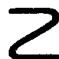
\includegraphics[keepaspectratio]{images/part001_8adf5445.jpg}}

and \(\operatorname{long}(\mathbf{M} / \mathfrak{q}\mathbf{M})\leqslant \operatorname{long}(\mathbf{M} / \mathfrak{x}\mathbf{M})\) ; the three cases

\[
e _ {\mathfrak {q}} (\mathrm{M}) <   \operatorname{long} (\mathrm{M} / \mathfrak {q} \mathrm{M}), e _ {\mathfrak {q}} (\mathrm{M}) = \operatorname{long} (\mathrm{M} / \mathfrak {q} \mathrm{M}), e _ {\mathfrak {q}} (\mathrm{M}) > \operatorname{long} (\mathrm{M} / \mathfrak {q} \mathrm{M})
\]

are possible (p.~106, exerc. 16 and 17).

